\graphicspath{
    {figures_and_references/fragility_curves/}
    {figures_and_references/EELISA_conference/}
}

% \selectlanguage{english}
\renewcommand{\chapternametext}{Chapter \thechapter . Use case: Generation of capacity curves with machine learning in the 3 pilot regions}
\renewcommand{\shortchapternametext}{Chapter \thechapter . Use case: Capacity curve generation}

\begin{refsection}

\chapter{\chapternametext}
\

\renewcommand{\headingtextL}{}
\renewcommand{\headingtextR}{\shortchapternametext}
\begingroup
 \flushbottom
 \setlength{\parskip}{0pt plus 1fil}%
 \localtableofcontents 
\endgroup
 
\begingroup
 \flushbottom
 \setlength{\parskip}{0pt plus 1fil}%
 \locallistoffigures
 \locallistoftables
\endgroup


\newpage

\setcounter{section}{0} 

\FloatBarrier

\renewcommand{\sectionnametext}{Finite element model}
\renewcommand{\headingtextL}{\shortchapternametext}
\renewcommand{\headingtextR}{\thesection. \sectionnametext}
\section{\sectionnametext}

To establish a baseline for structural performance, the open-source program OpenSees was utilized by our research team to conduct non-linear static "pushover" analyses \footcite{yepes-estrada_modeling_2017,jimenez-martinez_methodology_2024}. These simulations were performed on a suite of idealized masonry building models, systematically modified to capture the variability inherent in urban building stocks. The following structural and geometric variables were controlled across the simulations:

\begin{itemize}
    \item \textbf{Number of storeys:} Ranging from low to mid-rise configurations.
    \item \textbf{Relative position within the block:} Isolated, corner, edge, or central units.
    \item \textbf{Eccentricity:} Variations in $x$ and $y$ directions through the internal arrangement of partition walls.
    \item \textbf{Diaphragm type:} Modeling of both flexible and rigid roof diaphragms.
\end{itemize}

A total of 80 unique masonry building configurations were simulated (fig. \ref{fig:FEM}), and the resulting pushover curves were compiled into a standardized dataset. To ensure traceability, each curve was saved using a naming convention: 

\scalebox{0.9}{\small \texttt{\{floors\}-\{position\}-\{diaphragm\}-\{direction\}-\{asym\_x\}-\{asym\_y\}-\{unit\_L\}\_\{\{unit\_C\}\_\{\{unit\_R\}.txt} }

In this convention, each token (e.g., \texttt{NdXY}) represents a specific dwelling unit within an aggregate, where $N$ denotes the number of storeys, $d$ indicates the diaphragm type (R for rigid, F for flexible), and $X, Y$ represent the levels of structural asymmetry. For isolated dwellings, the descriptor is replaced by \texttt{ISOL\_ISOL\_ISOL}.

\renewcommand{\sectionnametext}{Machine learning model}
\renewcommand{\headingtextR}{\thesection. \sectionnametext}
\section{\sectionnametext}

Given the high computational cost of finite element modeling, it is not feasible to simulate every possible structural permutation. To overcome this limitation, a surrogate machine learning model was developed to predict the pushover response for arbitrary configurations not explicitly present in the original dataset. The model was trained using 60 representative samples and validated against a held-out test set of 20 samples.

The workflow begins by parsing the raw simulation output files and interpolating all curves to a fixed displacement length, ensuring consistency across tensors. The core of the predictive engine employs a combination of Principal Component Analysis (PCA) and Gaussian Process Regression (GPR). 

Gaussian Process Regression \footcite{rasmussen2003gaussian} is a powerful, non-parametric Bayesian approach for regression. Unlike deep learning approaches, which typically provide a single deterministic output, GPR operates within a Bayesian framework. This allows the model to output a posterior distribution for every prediction, providing an explicit estimate of the model's error and confidence levels. This capability is a significant advantage in seismic engineering: the error estimates provided by the Bayesian approach are essential for the subsequent development of fragility curves, as they allow for the quantification of uncertainty in the structural response. The "learning" process consists of determining the hyperparameters of a kernel function (such as the Matérn kernel used in this study), which defines the smoothness and correlation between input data points. 

In our pipeline, high-dimensional pushover curves are compressed via PCA into a reduced set of principal components. Independent GPR models are then trained for each component. Furthermore, a "conservative bias" correction factor of 0.05 was incorporated into the regression. This introduces a controlled safety margin, ensuring that in regions of high uncertainty, the predicted capacity is shifted toward more conservative (lower) estimates, which is a standard precaution in seismic risk engineering to avoid overestimating structural resistance when generating structural fragility models.

\renewcommand{\sectionnametext}{Results}
\renewcommand{\headingtextR}{\thesection. \sectionnametext}
\section{\sectionnametext}

The performance of the predictive model was evaluated through multiple experiments using various hyperparameters. The results for the most successful experiment are summarized in Table \ref{tab:gpr_results}.

\begin{table}[htbp]
\centering
\begin{tabular}{|l|c|c|c|}
\hline
\textbf{Metric} & \textbf{Without Bias Correction} & \textbf{With Conservative Bias} \\ \hline
$R^2$ Score     & 0.795                            & 0.776                          \\ \hline
RMSE            & 0.161                            & 0.168                          \\ \hline
MAE             & 0.097                            & 0.107                          \\ \hline
$\%$ Below      & 51.0\%                           & 72.1\%                         \\ \hline
\end{tabular}
\caption{Performance metrics for the GPR model.}
\label{tab:gpr_results}
\end{table}

The model demonstrates significant predictive capability. Representative samples of the predicted curves versus the ground truth are shown in figure \ref{fig:some_curves}. The visual comparison confirms that the majority of the predicted curves fall well within the 1-$\sigma$ error bounds, proving the validity of the methodology. 

A notable exception was identified in the \texttt{1R11\_3R11\_1R11} configuration (fig. \ref{fig:all_curves}), where the model overestimated the capacity beyond the 2-$\sigma$ threshold. This discrepancy is attributed to the lack of similar configurations in the training dataset. This finding is analytically valuable: it serves as a "sampling guide," identifying specific building configurations that are currently under-represented. Future iterations will prioritize these architectures for high-fidelity finite element simulation to further enrich the training dataset and improve global model reliability.

\begin{figure}[htbp]
    \centering
    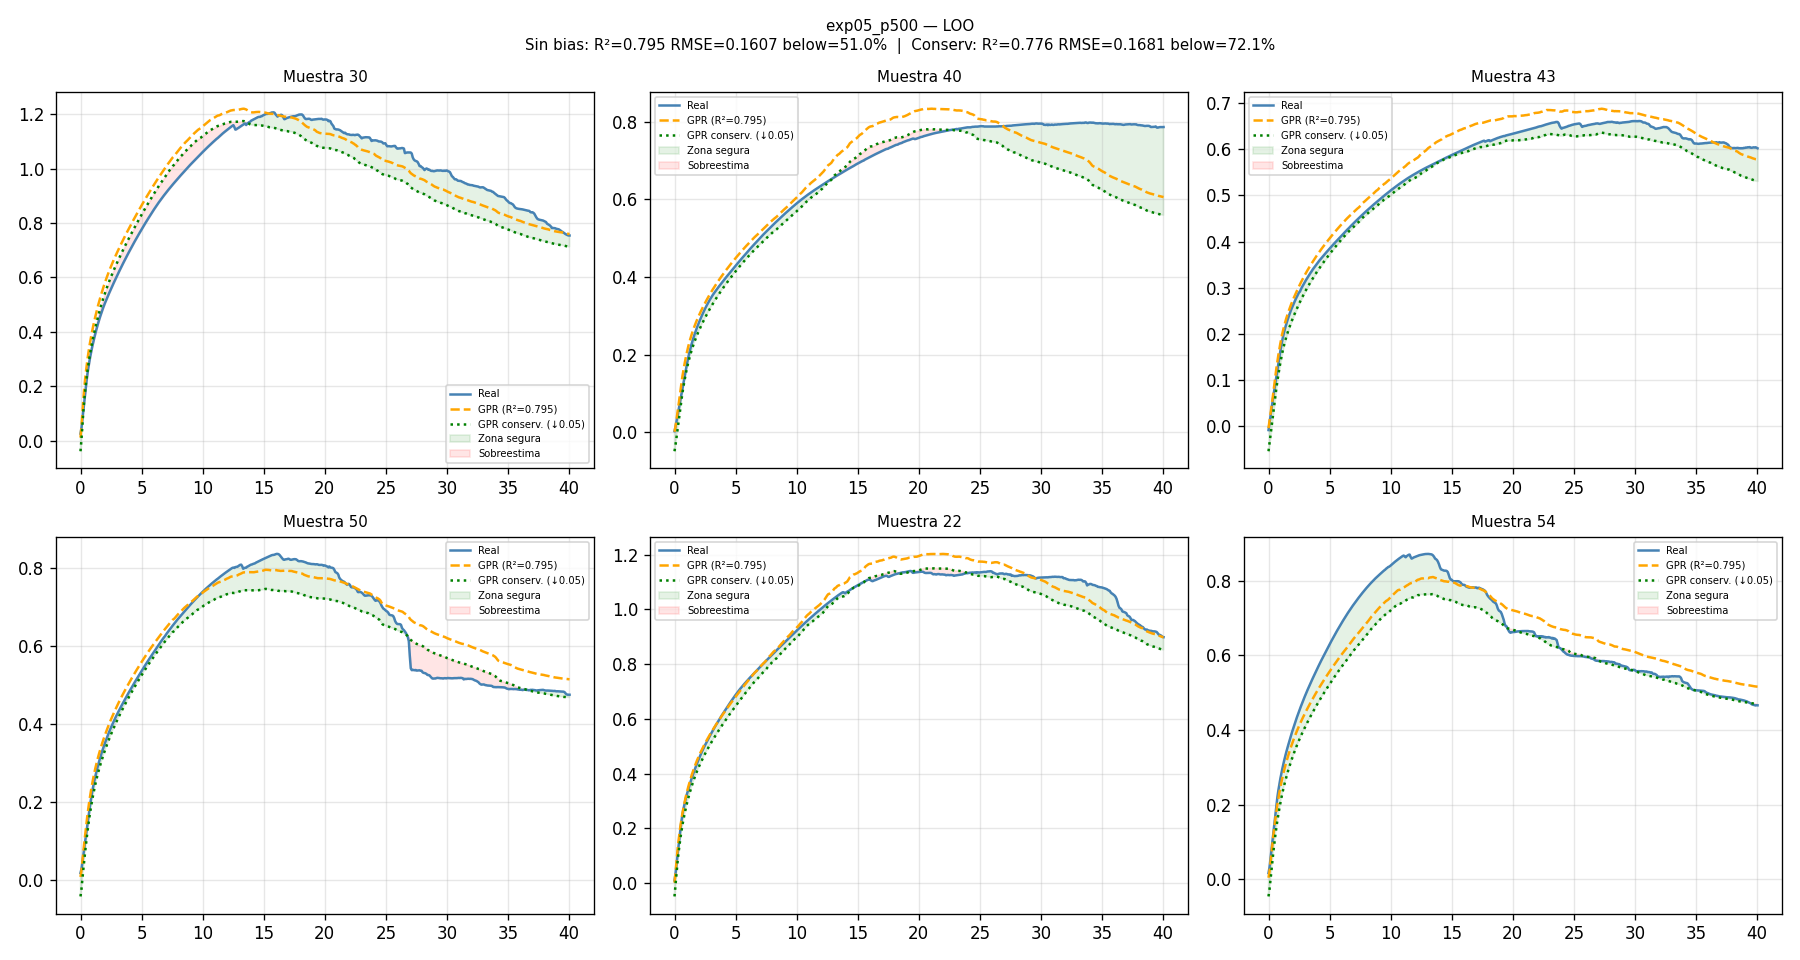
\includegraphics[width=0.8\textwidth]{figures/some_curves.png}
    \caption{Comparison of predicted versus simulated pushover curves for selected configurations.}
    \label{fig:some_curves}
\end{figure}

\begin{figure}[htbp]
    \centering
    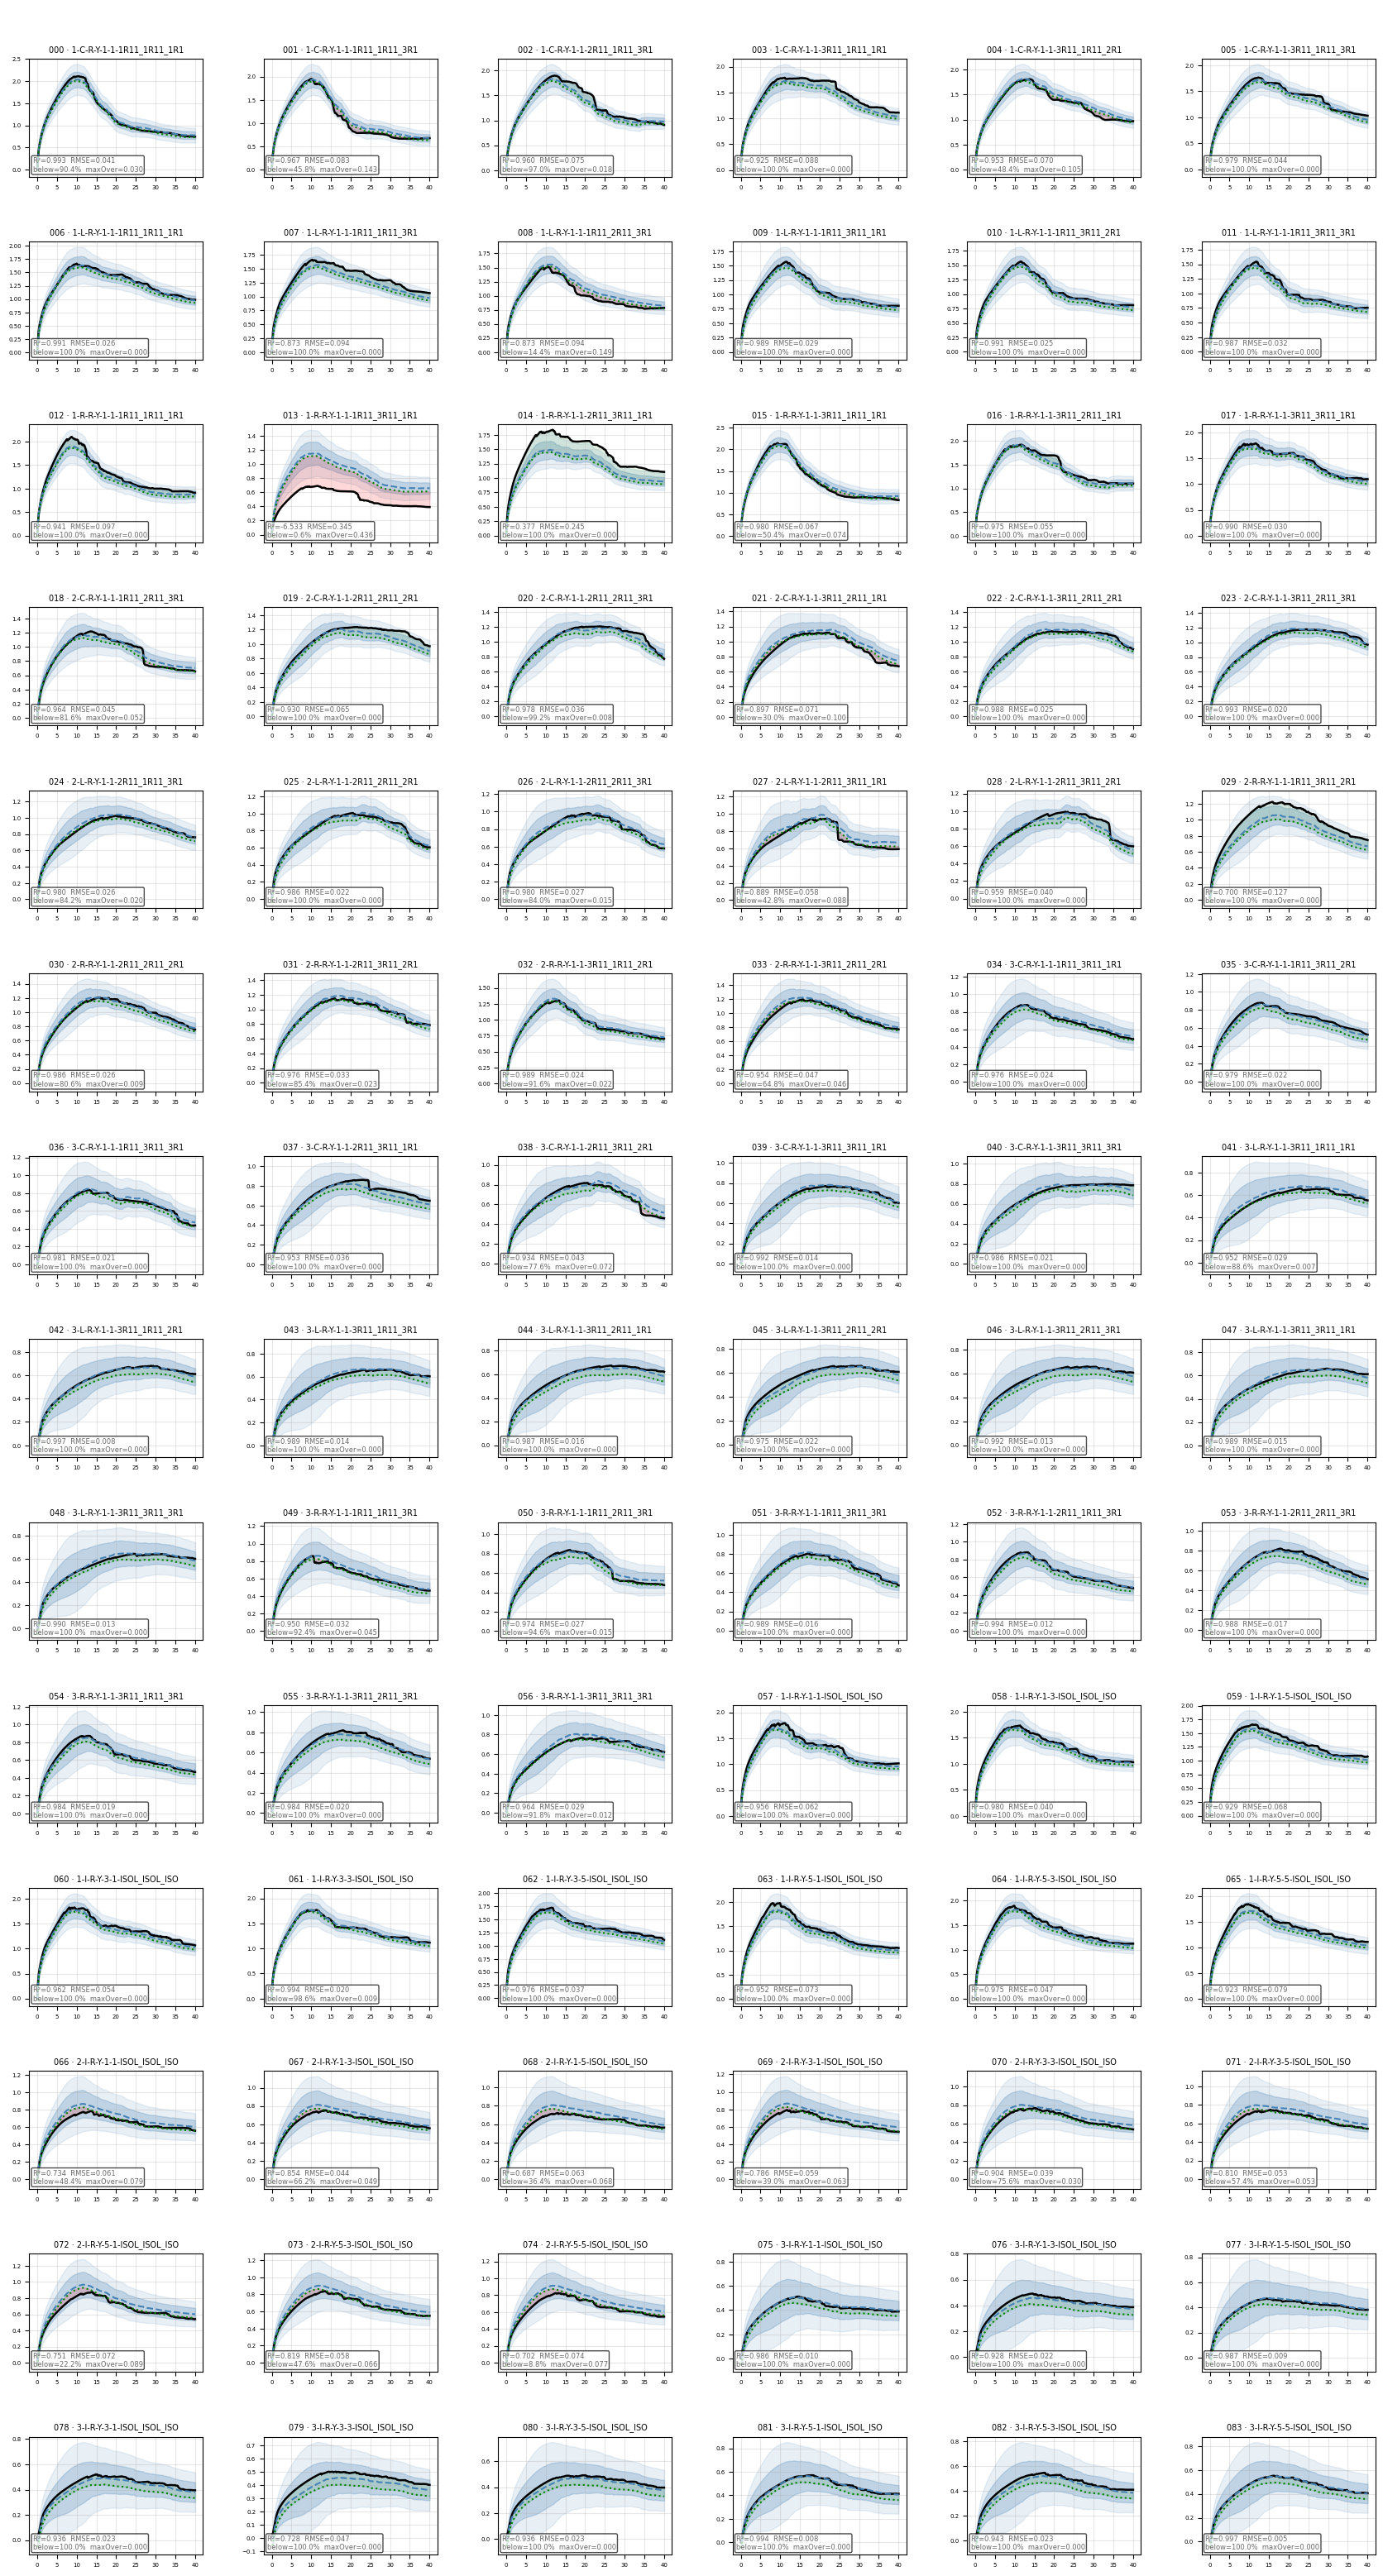
\includegraphics[width=0.8\textwidth]{figures/all_curves.png}
    \caption{All predicted capacity curves from the train and test sets.}
    \label{fig:all_curves}
\end{figure}

\newpage

\FloatBarrier

\renewcommand{\sectionnametext}{References}
\renewcommand{\headingtextR}{\thesection. \sectionnametext}
\section{\sectionnametext}
\printbibliography[heading=none]

\end{refsection}